\documentclass[usenames,dvipsnames]{beamer}

\mode<presentation>
{
  \usetheme{CambridgeUS}
  \usecolortheme{orchid}
  \setbeamercovered{transparent}
  \useinnertheme{rectangles}
  \setbeamertemplate{navigation symbols}{}
  \usefonttheme[onlymath]{serif}
  \setbeamercolor{title}{bg=alerted text.fg!85!black, fg=white}
  \setbeamercolor{item projected}{bg=alerted text.fg!85!black}
  \setbeamertemplate{enumerate items}[default]
  \setbeamercolor{local structure}{fg=alerted text.fg!85!black}
  \setbeamersize{text margin left=0.2cm,text margin right=0.2cm}
}

\newcommand\Shorter[2][1]{%
\makebox[\linewidth][c]{%
  \begin{minipage}{\dimexpr\textwidth+#1\relax}
  \raggedright#2
  \end{minipage}%
  }%
}
\usepackage[english]{babel}
\usepackage[utf8]{inputenc}
\usepackage[T1]{fontenc}
\usepackage{lmodern}
\usepackage{pifont}
\usepackage{mathrsfs}
\usepackage{amsmath}
\usepackage{bm}
\usepackage{caption}
\usepackage{subcaption}
\usepackage{outlines}
\usepackage{booktabs}
\usepackage{minted}
\usepackage[listings, minted]{tcolorbox}
\tcbset{left=6mm}
\usepackage[%
autocite     = plain,
doi          = true,
url          = true,
giveninits   = true,
hyperref     = true,
backref      = true,
maxbibnames  = 99,
maxcitenames = 99,
sortcites    = true,
style        = authoryear,
]{biblatex}

\addbibresource{presentation.bib}

\newcommand{\fakeimage}{{\fboxsep=-\fboxrule\fbox{\rule{0pt}{3cm}\hspace{4cm}}}}

\usepackage{tikz}
\usetikzlibrary{quotes}
\usetikzlibrary{bayesnet}
\usetikzlibrary{arrows,calc,positioning,decorations.pathreplacing}
\tikzset{
  >=stealth',
  punkt/.style={
    circle,
    draw=black, thick,
    minimum height=1.75em,
    inner sep=0pt,
    text centered},
  pil/.style={
    ->,
    thick}
}

\definecolor{isabelline}{rgb}{0.96, 0.94, 0.93}
\definecolor{palesilver}{rgb}{0.79, 0.75, 0.73}
\definecolor{hdblue}{HTML}{3366cc}
\hypersetup{colorlinks,linkcolor=,urlcolor=hdblue, citecolor=hdblue}

\setminted{highlightcolor=black!5, linenos}
\setminted{style=emacs}
\setminted{bgcolor=isabelline}
\setminted{fontsize=\fontsize{4.5}{1}\selectfont}
\setminted{highlightcolor=palesilver}
\renewcommand{\theFancyVerbLine}{{\fontsize{4}{1}\selectfont \arabic{FancyVerbLine}}}

\newcommand{\xmark}{\ding{55}}
\newcommand{\highlight}[1]{%
  \colorbox{blue!20}{$\displaystyle#1$}}


\def\ci{\perp\!\!\!\perp}
\makeatletter
\newcommand*{\indep}{%
  \mathbin{%
    \mathpalette{\@indep}{}%
  }%
}
\newcommand*{\nindep}{%
\mathbin{%                   % The final symbol is a binary math operator
  \mathpalette{\@indep}{\not}% \mathpalette helps for the adaptation
  % of the symbol to the different math styles.
}%
}
\def\layersep{.38cm}
\def\inlsep{.4}
\newcommand*{\@indep}[2]{%
% #1: math style
% #2: empty or \not
  \sbox0{$#1\perp\m@th$}%        box 0 contains \perp symbol
  \sbox2{$#1=$}%                 box 2 for the height of =
  \sbox4{$#1\vcenter{}$}%        box 4 for the height of the math axis
  \rlap{\copy0}%                 first \perp
  \dimen@=\dimexpr\ht2-\ht4-.2pt\relax
  % The equals symbol is centered around the math axis.
  % The following equations are used to calculate the
  % right shift of the second \perp:
  % [1] ht(equals) - ht(math_axis) = line_width + 0.5 gap
  % [2] right_shift(second_perp) = line_width + gap
  % The line width is approximated by the default line width of 0.4pt
  \kern\dimen@
  {#2}%
  % {\not} in case of \nindep;
  % the braces convert the relational symbol \not to an ordinary
  % math object without additional horizontal spacing.
  \kern\dimen@
  \copy0 %                       second \perp
}
\makeatother


\title[MultiVerse]{MultiVerse: Causal Reasoning Using Importance Sampling in Probabilistic Programming}

% \subtitle
% {Presentation Subtitle} % (optional)

\author[Dogan]
{%
\texorpdfstring{
  \begin{columns}
    \column{.85\linewidth}
    \centering
    Presented by:\\
    Haluk Dogan\\
    \url{https://haluk.github.io/}\\
    \href{mailto:hdogan@vivaldi.net}{hdogan@vivaldi.net} \\
    Some slides copied from \\
    Frank Wood
  \end{columns}
}
{Dogan}
}
\institute[UNL] % (optional, but mostly needed)
{
  Department of Computer Science\\
  University of Nebraska-Lincoln
}

\date[\today] % (optional)
{\today}

\subject{Talks}

\pgfdeclareimage[height=0.5cm]{university-logo}{figures/logo}
\logo{\pgfuseimage{university-logo}}

\begin{document}

\begin{frame}[noframenumbering,plain]
  \titlepage{}
\end{frame}

\section{Introduction}\label{sec:introduction}
\begin{frame}
  \frametitle{Probabilistic Programming Languages (PPL)}
  \begin{figure}[ht]
    \centering
    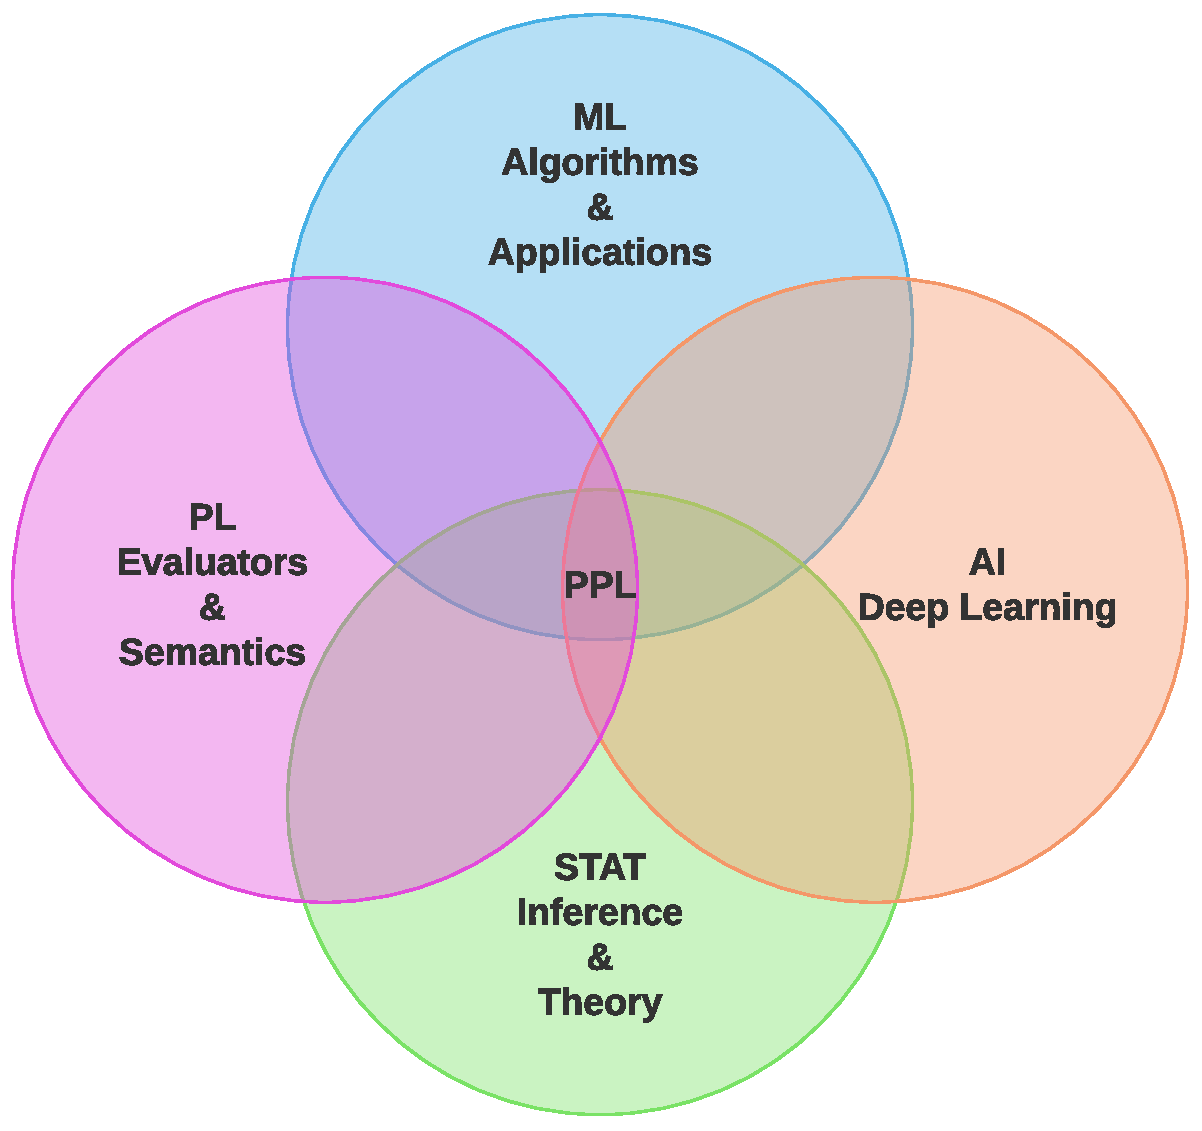
\includegraphics[width=0.65\textwidth,keepaspectratio]{figures/pplvenn.pdf}
    \caption*{\label{fig:ppl-venn}}
  \end{figure}
\end{frame}
\begin{frame}
  \frametitle{Intuition}
  \begin{figure}[ht]
    \centering
    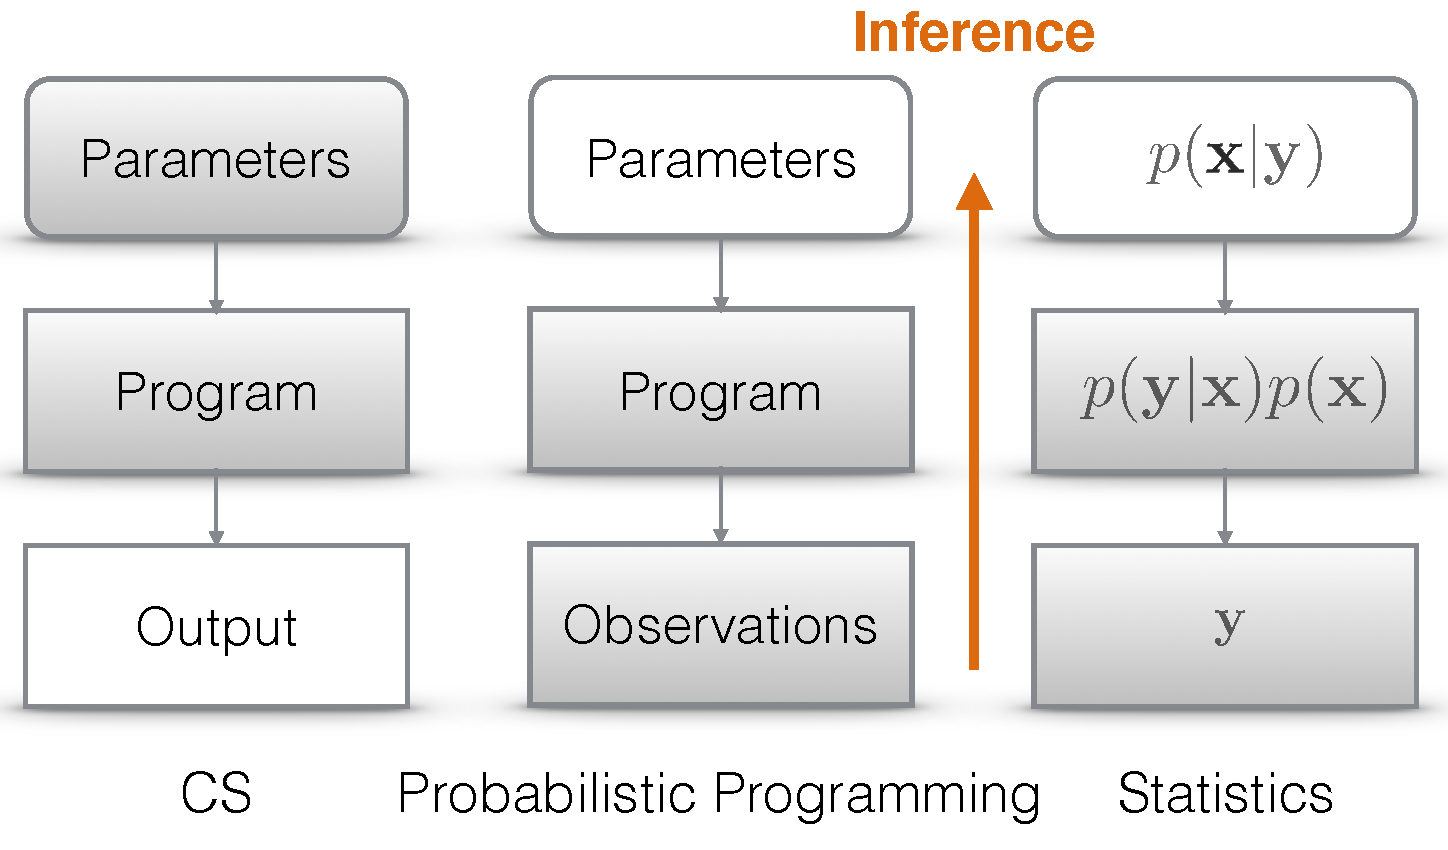
\includegraphics[height=0.7\textheight,keepaspectratio]{figures/ppl_similarity.pdf}
    \caption*{\label{fig:ppl-similarity}}
  \end{figure}
\end{frame}
\begin{frame}
  \frametitle{The Way Machine Learning Is}
  \begin{figure}[ht]
    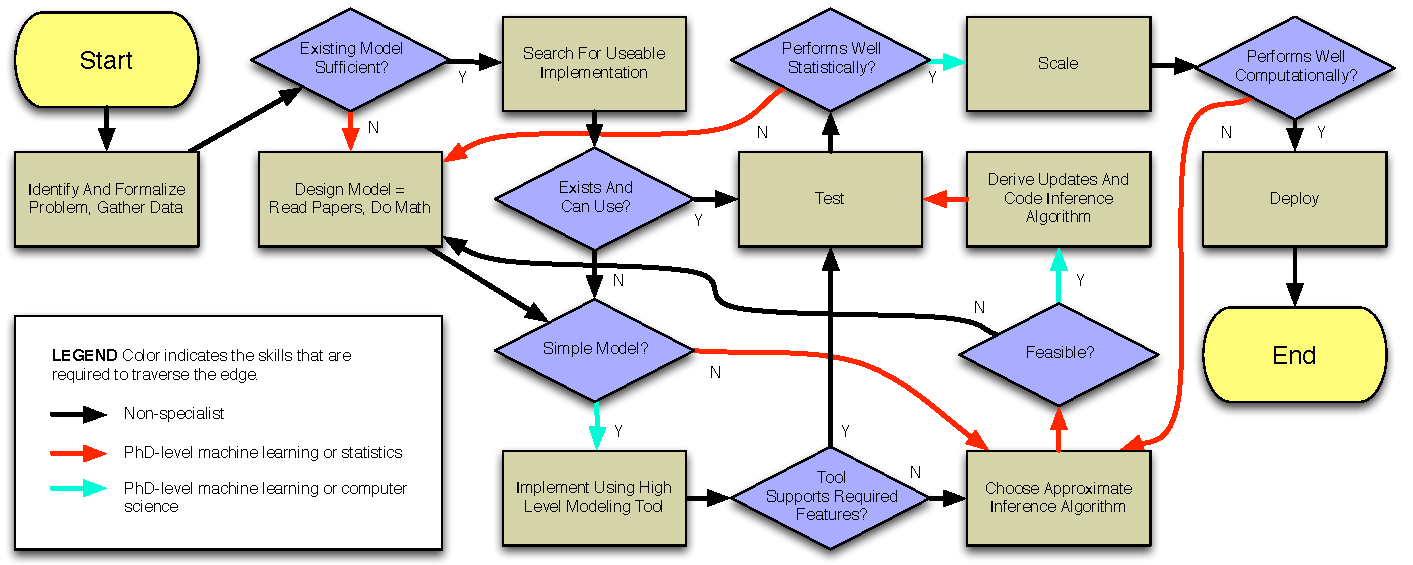
\includegraphics[width=1\textwidth,keepaspectratio]{figures/ml_current.pdf}
    \caption*{\label{fig:ml-current}}
  \end{figure}
\end{frame}
\begin{frame}
  \frametitle{The Way Machine Learning Will Be }
  \begin{figure}[ht]
    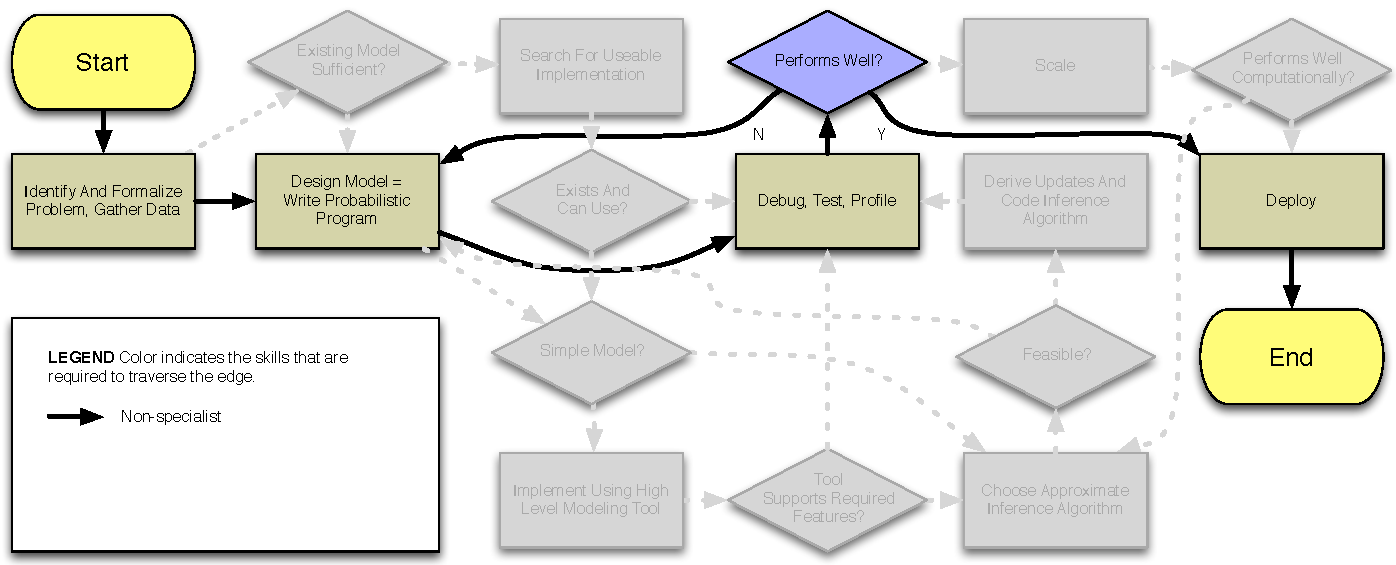
\includegraphics[width=1\textwidth,keepaspectratio]{figures/ml_future.pdf}
    \caption*{\label{fig:ml-future}}
  \end{figure}
\end{frame}
\begin{frame}
  \frametitle{Causality}
  \begin{columns}
    \begin{column}[t]{.48\textwidth}
      \begin{figure}[ht]
        \centering
        \vspace{-0.8cm}
        \hspace{-1.5cm}
        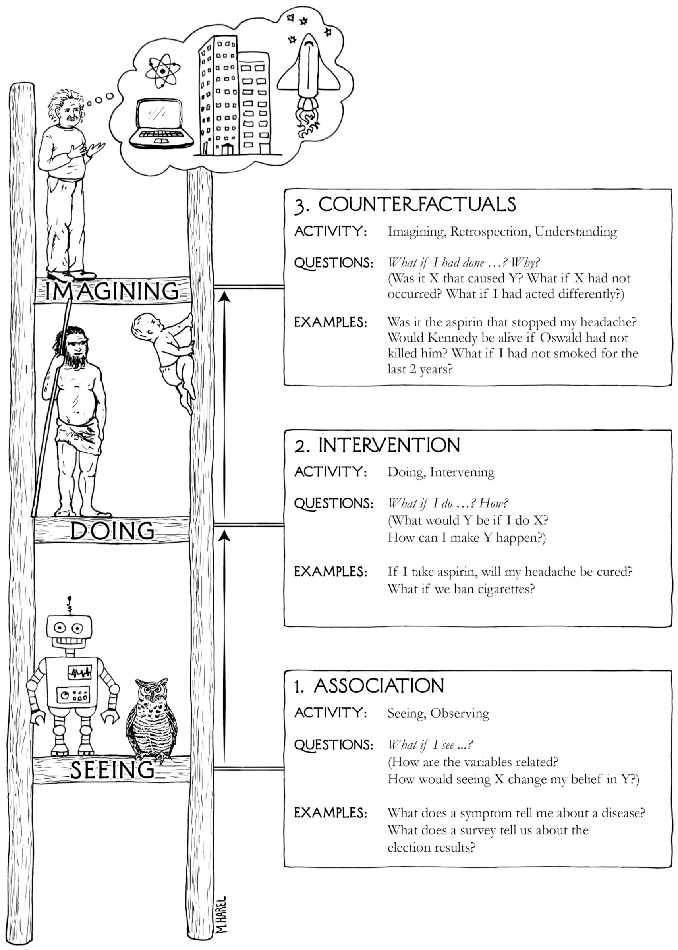
\includegraphics[height=0.8\textheight,keepaspectratio]{figures/ladder_of_causation.png}
        \caption*{\tiny{Ladder of Causation~\parencite{JudeaPearl2018}}\label{fig:ladder-causation}}
      \end{figure}
    \end{column}
    \hspace{-2cm}
    \begin{column}[t]{.50\textwidth}
      Causal Model $M(X,Y,F)$:
      \begin{itemize}
        \item $X$: Exogenous variables (latent)
        \item $Y$: Endogenous variables (observed)
        \item $F$: Set of structural equations $\left\{F_{K} \mid K \in Y\right\}$
      \end{itemize}
      \vspace{0.2cm}
      Counterfactual inference query:\vspace{-0.2cm}
      \[
        P(Y' \mid Y = e; \text{do}(D = d))
      \]
      Evaluating this query in 3 steps:
      \begin{itemize}
        \item Abduction \begin{tiny}(observational inference)\end{tiny}
        \item Intervention \begin{tiny}(action)\end{tiny}
        \item Prediction
      \end{itemize}
    \end{column}
  \end{columns}
\end{frame}
\begin{frame}
  \frametitle{Abduction and Counterfactual Inference}
  Abduction
  \begin{itemize}
    \item The hardest part of the counterfactual procedure
      \begin{itemize}
        \item Exact inference is possible but either difficult or intractable
      \end{itemize}
    \item $M' \leftarrow P(X \mid Y=e)$
      \begin{itemize}
        \item It has the same structure as model $M$
        \item $X$ is replaced by $X \mid Y=e$
        \item $Y$ is not observed anymore
      \end{itemize}
  \end{itemize}
  Counterfactual inference
  \begin{itemize}
    \item Twin-net approach, i.e., loopy belief propagation \parencite{Balke1994}
    \item Single-world intervention graphs \parencite{Richardson2013}
    \item Matching \parencite{Li2012}
  \end{itemize}
\end{frame}
\begin{frame}
  \frametitle{Importance Sampling}
  \begin{itemize}
    \item Approximate inference technique
      \[\mathbb{E}[f(x)]=\int f(x) p(x) d x \approx \frac{1}{n} \sum_{i} f\left(x_{i}\right)\]
    \item If sampling from $p(x)$ is very hard
      \[\mathbb{E}[f(x)]=\int f(x) p(x) d x=\int \highlight{f(x) \frac{p(x)}{q(x)}} q(x) d x \approx \frac{1}{n} \sum_{i} f\left(x_{i}\right) \frac{p\left(x_{i}\right)}{q\left(x_{i}\right)}\]
    \item $\sigma^{2}(X)=\mathbb{E}[X^{2}]-{\mathbb{E}[X]}^{2}$
  \end{itemize}
\end{frame}
\begin{frame}[fragile]
  \frametitle{Continuous Variable Example in MultiVerse}
\Shorter[-0.8cm] {
  \begin{columns}
    \begin{column}{.63\textwidth}
      \inputminted[autogobble, highlightlines={29}]{python3}{src/ex1.py}
    \end{column}
    \begin{column}{.35\textwidth}
      \begin{figure}[ht]
        \scalebox{0.7}{\input{figures/gaussian_model.tikz}}
        \caption*{\label{fig:gaussian-model}}
      \end{figure}
      \hspace{-0.3cm}
      \tiny{
        $\mathbb{E}(Y' \mid Y=1.2342,\text{do}(Z=-2.5236))$
      }
    \end{column}
  \end{columns}
}
\end{frame}
\begin{frame}[fragile]
  \frametitle{Continuous Variable Example in Pyro}
  \Shorter[-0.8cm] {
    \inputminted[autogobble, lastline=31]{python3}{src/ex1_pyro.py}
  }
\end{frame}
\begin{frame}[fragile]
  \frametitle{Continuous Variable Example in Pyro (cont'd)}
  \Shorter[-0.8cm] {
    \inputminted[autogobble, firstline=32, lastline=61]{python3}{src/ex1_pyro.py}
  }
\end{frame}
\begin{frame}[fragile]
  \frametitle{Continuous Variable Example in Pyro (cont'd)}
  \Shorter[-1cm] {
    \inputminted[autogobble, firstline=62]{python3}{src/ex1_pyro.py}
  }
\end{frame}

\section{Experiments}\label{sec:experiments}
\begin{frame}
  \frametitle{Experiments}
  \begin{itemize}
    \item 16-core EC2 instance m4.4xlarge
    \item 1000 SCM with 15 probabilistic procedures
      \begin{itemize}
        \item BNs in the form of probabilistic programs
      \end{itemize}
    \item MultiVerse experiments
      \begin{itemize}
        \item produce the same number of samples in less time than Pyro
        \item have better inference convergence
      \end{itemize}
  \end{itemize}
\end{frame}
\begin{frame}
  \frametitle{Test Models}
  \begin{figure}[ht]
    \input{figures/example_model.tikz}
    \caption*{\label{fig:example-model}}
  \end{figure}
\end{frame}
\begin{frame}
  \frametitle{Time Performance Comparison}
  \begin{columns}
    \begin{column}{.48\textwidth}
      \begin{figure}[ht]
        \centering
        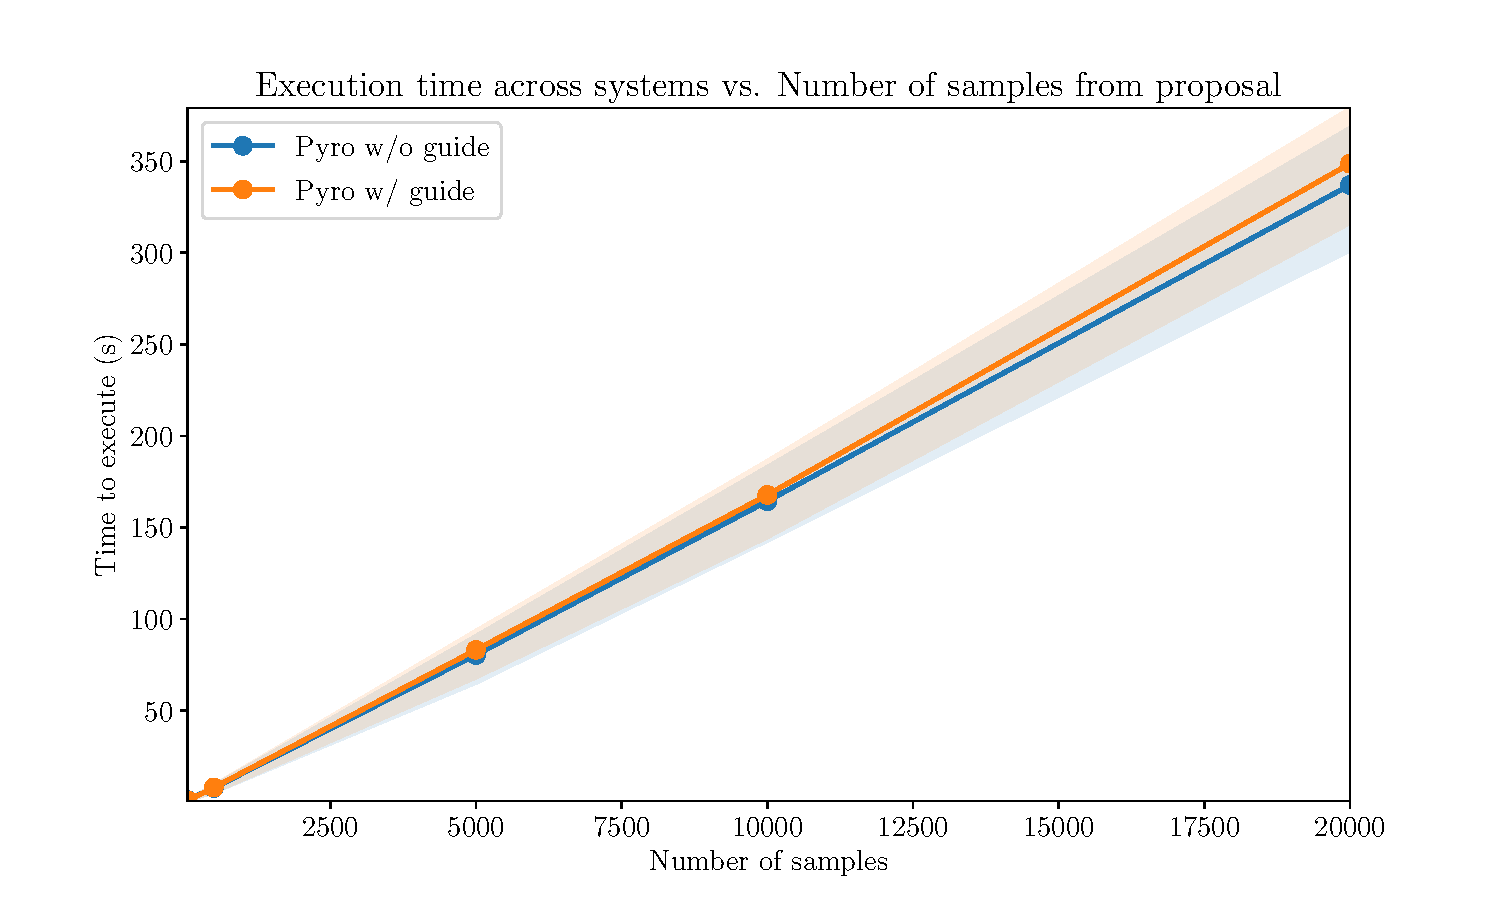
\includegraphics[width=1.0\textwidth,height=0.6\textheight]{figures/times0.pdf}
        \caption*{\label{fig:pyro-time}}
      \end{figure}
    \end{column}
    \begin{column}{.48\textwidth}
      \begin{figure}[ht]
        \centering
        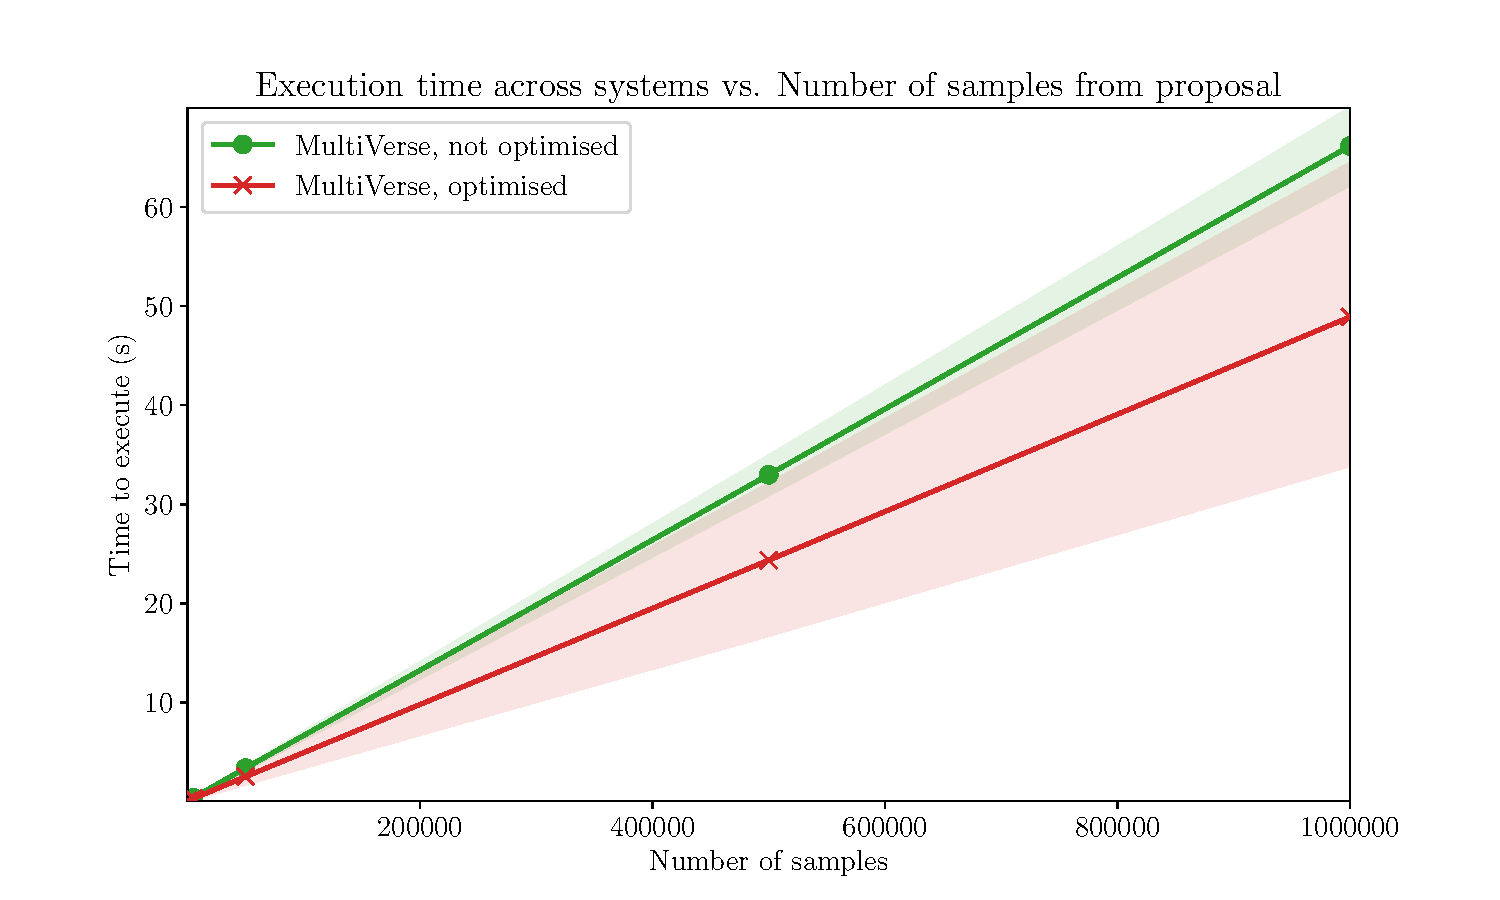
\includegraphics[width=1.0\textwidth,height=0.6\textheight]{figures/times1.pdf}
        \caption*{\label{fig:multiverse-time}}
      \end{figure}
    \end{column}
  \end{columns}
\end{frame}
\begin{frame}
  \frametitle{Convergence Test Performance}
  \begin{figure}[ht]
    \centering
    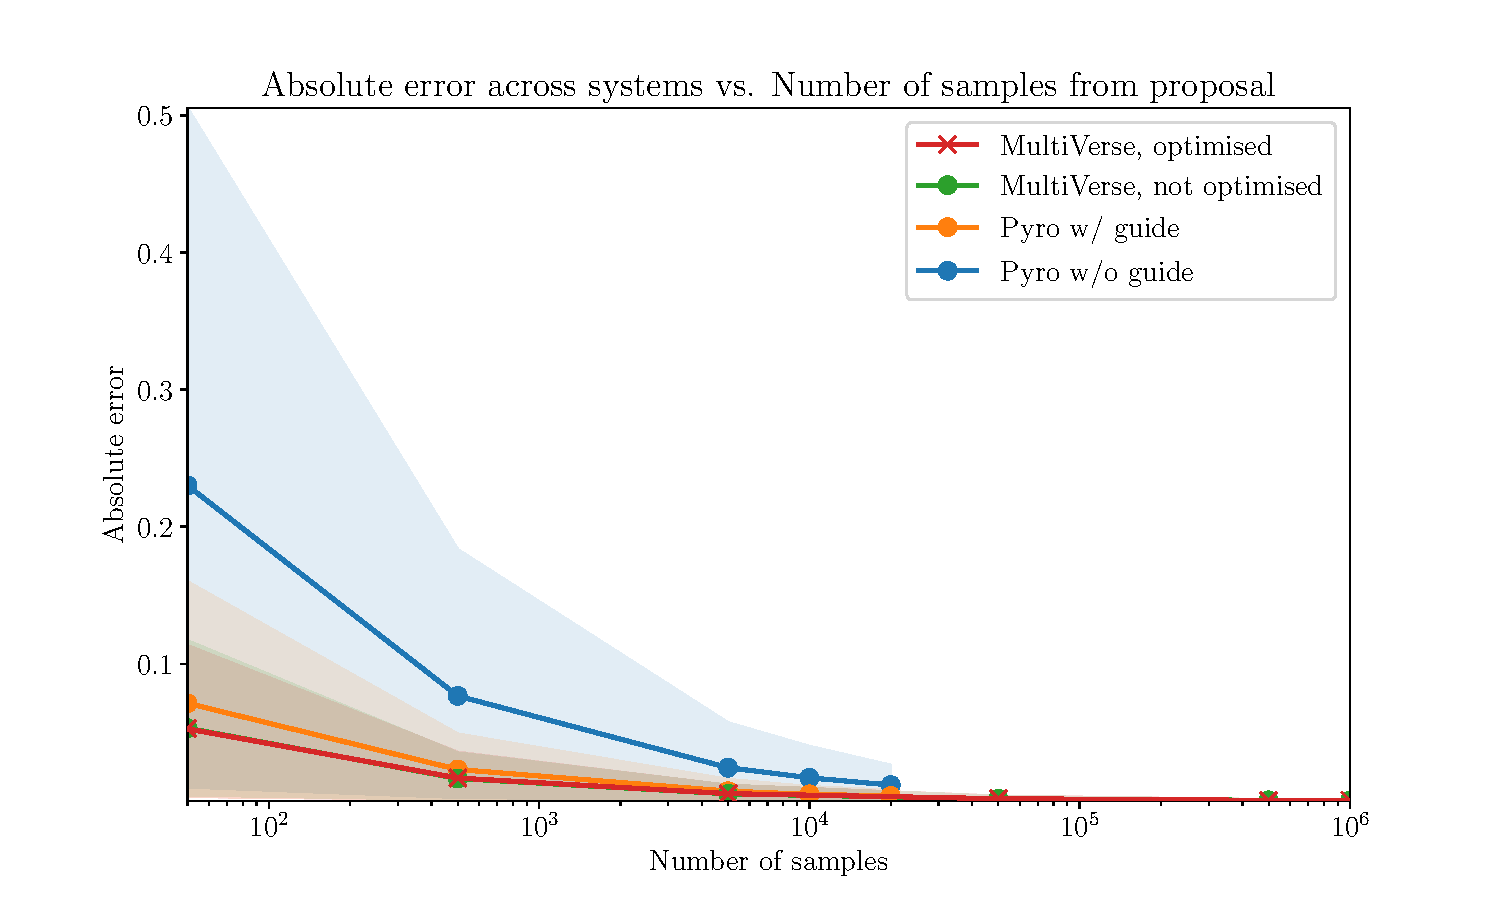
\includegraphics[width=1.0\textwidth,keepaspectratio]{figures/convergence.pdf}
    \caption*{\label{fig:convergence}}
  \end{figure}
\end{frame}
\section{Conclusion}
\begin{frame}[fragile]
  \frametitle{PPL Should Be Pure Functional}
  Anglican
  \begin{minted}[fontsize=\normalsize,autogobble]{clojure}
     [assume (a (normal 5 10))]
     [assume (b (normal a 2))]
     [assume (a (normal b 7))]
     => Error
  \end{minted}
  Probabilistic-C
  \begin{minted}[fontsize=\normalsize,autogobble]{c}
     int a = normal(5, 10);
     int b = normal(a, 2);
     int a = normal(b, 7);
  \end{minted}
\end{frame}
\begin{frame}[fragile]
  \frametitle{Birthday Paradox}
  Approximately, what's the probability that in a room filled with 23 people at
  least one pair of people have the same birthday?
  \begin{minted}[fontsize=\small,autogobble]{clojure}
     [assume birthday (mem (lambda (i) (uniform-discrete 1 366)))]

     [assume N 23]

     [assume pair-equal
       (lambda (i j)
         (if (> i N)
           false
           (if (> j N)
             (pair-equal (+ i 1) (+ i 2))
               (if (= (birthday i) (birthday j))
                 true
                 (pair-equal i (+ j 1))))))]

     [predict (pair-equal 1 2)]
  \end{minted}
\end{frame}
\begin{frame}
  \frametitle{Questions}
  \begin{center}
    \Huge{Questions?}
  \end{center}
  \begin{figure}
    \centering
    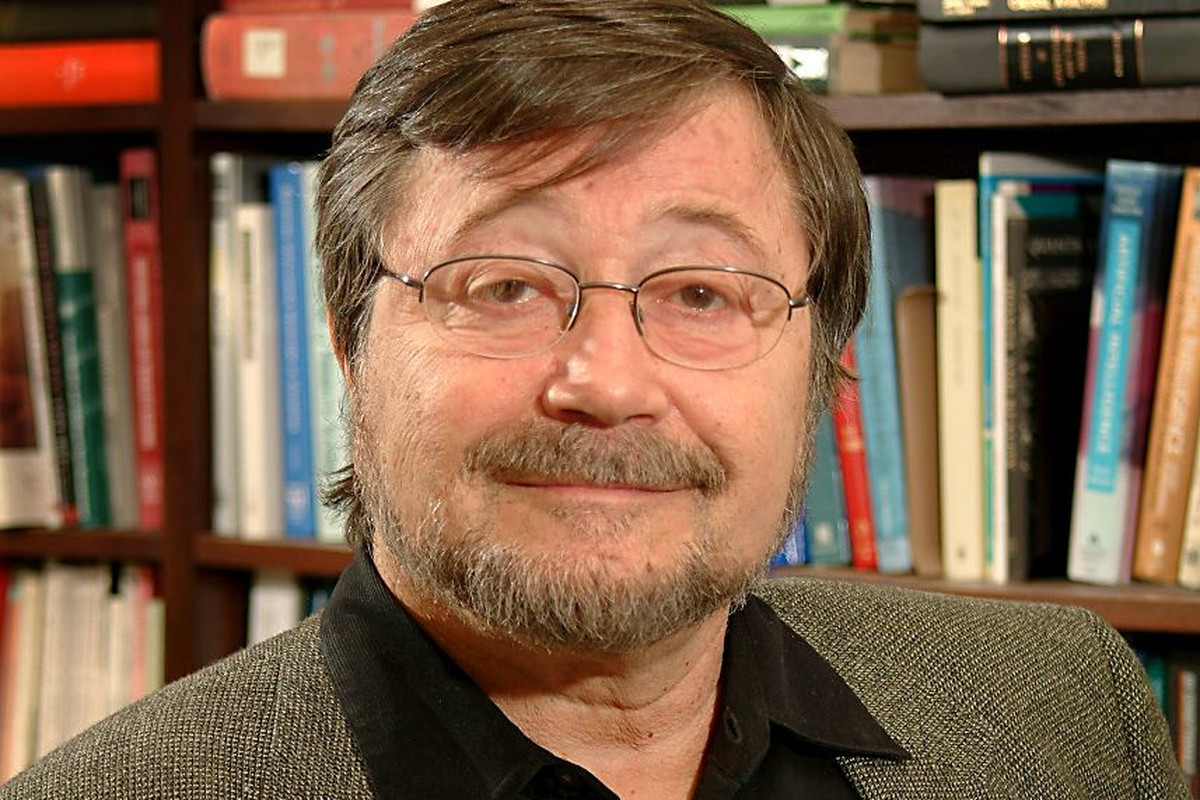
\includegraphics[width=0.7\textwidth, height=0.6\textheight]{figures/judeapearl.png}
    \caption*{Judea Pearl, winner of Turing Award (2011)}
  \end{figure}
\end{frame}
\begin{frame}[allowframebreaks]
  \frametitle{References}
  \printbibliography{}
\end{frame}
\end{document}

%%% Local Variables:
%%% mode: latex
%%% TeX-master: t
%%% End:
